\documentclass[handout, 9pt]{beamer}

%!TEX root = ../notas_de_clase.tex

%preamble

%language
\usepackage[spanish,es-nodecimaldot]{babel}
\usepackage[utf8]{inputenc}
\usepackage{apacite}
\usepackage[absolute,overlay]{textpos}

%packages
\usepackage[Algoritmo]{algorithm}
\usepackage{algorithmicx}
\usepackage[noend]{algpseudocode}
\usepackage{mathtools}
\setlength {\marginparwidth}{2cm}
\usepackage{todonotes}
\usepackage{amsbsy}
\usepackage{amssymb}
\usepackage{amsmath,bm}
\usepackage{dsfont}

\usepackage{xcolor}
\providecommand{\sred}[1]{\textcolor{red}{#1}}
\providecommand{\sblue}[1]{\textcolor{blue}{#1}}
\providecommand{\red}[1]{\textcolor{red}{\text{#1}}}
\providecommand{\blue}[1]{\textcolor{blue}{\text{#1}}}
\providecommand{\redb}[1]{\textcolor{red}{\textbf{#1}}}
\providecommand{\blueb}[1]{\textcolor{blue}{\textbf{#1}}}
\usepackage{graphicx}
\usepackage{fancybox}
\usepackage{booktabs}
\usepackage{caption}
\usepackage{float}
%\usepackage[longend,ruled,algochapter,linesnumbered,lined,boxed,commentsnumbered,spanish]{algorithm2e}
%\usepackage[algo2e]{algorithm2e}
\usepackage{amssymb}
\usepackage{amstext}
\usepackage{bm}
\usepackage{wrapfig}
\usepackage{subcaption} % para_unsupervised_chapter

%formatting

\usepackage[export]{adjustbox}

%caption para figuras
\captionsetup[figure]{width=.8\linewidth, font=small,labelfont={bf},name={Fig.},labelsep=period}
\captionsetup[table]{width=.8\linewidth,font=small,labelfont={bf},name={Tabla},labelsep=period}



\ifx\byn\undefined
    \definecolor{my_blue}{HTML}{C2D5FF}
    \definecolor{my_red}{HTML}{FFC2C2}
    \definecolor{my_yellow}{HTML}{FFFFE0}
\else
    \definecolor{my_blue}{HTML}{FFFFFF}
    \definecolor{my_red}{HTML}{FFFFFF}
    \definecolor{my_yellow}{HTML}{FFFFFF}
\fi


\usepackage[framemethod=TikZ]{mdframed}
\mdfdefinestyle{discusion}{%
    %linecolor=black,
    %outerlinewidth=0pt,
    roundcorner=0pt,
    innertopmargin=5pt,
    innerbottommargin=5pt,
    innerrightmargin=20pt,
    innerleftmargin=20pt,
    backgroundcolor=my_blue}

\colorlet{Green}{green!90}


\mdfdefinestyle{ejemplo}{%
    %linecolor=black,
    %outerlinewidth=0pt,
    roundcorner=0pt,
    innertopmargin=5pt,
    innerbottommargin=5pt,
    innerrightmargin=20pt,
    innerleftmargin=20pt,
    backgroundcolor=my_yellow}


\mdfdefinestyle{pendiente}{%
    style = discusion, 
    backgroundcolor=my_red}


\RequirePackage{url}



%definitions
\def\td{{\text d}}
\def\cN{{\mathcal N}}
\def\cX{{\mathcal X}} 
\def\cC{{\mathcal C}} 
\def\N{{\mathbb N}}
\def\d{{\text d}}
\def\datos{{\mathcal D}}
\def\eye{{\mathbb I}}
\def\ssum{{\scriptstyle\sum}}
\def\bepsilon{{\bm \epsilon}}
\def\tx{\tilde{x}}
\def\tX{\tilde{X}}
\def\thetaMAP{\theta_\text{MAP}}
\newcommand{\gp}{\ensuremath{\mathcal{GP}}}
\newcommand{\pr}{\ensuremath{\mathbb{P}}}
\newcommand{\x}{\ensuremath{\mathbf{x}}}
\newcommand{\z}{\ensuremath{\mathbf{z}}}
\newcommand{\cvector}{\ensuremath{\mathbf{c}}}
\newcommand{\e}{\ensuremath{\mathbf{e}}}
\newcommand{\y}{\ensuremath{\mathbf{y}}}
\newcommand{\bx}{\ensuremath{\textcolor{blue}{X}}}
\newcommand{\by}{\ensuremath{\textcolor{blue}{Y}}}
\newcommand{\rx}{\ensuremath{\textcolor{red}{X_*}}}

\newcommand{\R}{\mathbb{R}}
\newcommand{\norm}[1]{\left\lVert#1\right\rVert}




\DeclareMathOperator*{\argmax}{arg\,max}
\DeclareMathOperator*{\argmin}{arg\,min}
\DeclareMathOperator{\E}{\mathbb{E}}
\DeclareMathOperator{\V}{\mathbb{V}}
\DeclareMathOperator{\KL}{\text{KL}}
\DeclareMathOperator{\MVN}{\text{MVN}}
\newcommand\deq{\stackrel{\mathclap{\normalfont\mbox{\tiny def}}}{=}}
%\newcommand{\E}[1]{\mathbb E \left[#1\right]}
\newcommand{\trace}[1]{\text{Tr} \left[#1\right]}


\usepackage{amsthm}

%-------------------------------------------
% Newtheorem
%-------------------------------------------
\newtheorem{axioma}{\textcolor{red}{Axioma}}
\newtheorem{definicion}{Definición}
\newtheorem*{notacion}{Notación}
\newtheorem{teorema}{Teorema}
\newtheorem{corolario}{Corolario}
\newtheorem{lema}{Lema}
\newtheorem{lemaZ}{\textcolor{red}{Lema}}
\newtheorem{propiedad}{Propiedad:}
\newtheorem{proposicion}{Proposición:}
\newtheorem*{observacion}{Observación}
\newtheorem*{comentario}{Comentario}
\newtheorem*{ejemplo}{Ejemplo}
\newtheorem*{resultado}{Resultado}
\newtheorem*{propuesto}{Ejercicio propuesto}
\newtheorem*{demostracion}{Demostración} % No se usa, usar \begin{proof}\end{proof} que son por default.

%listing paackage para código
\usepackage{listings}
\usepackage{xcolor}
 
\definecolor{codegreen}{rgb}{0,0.6,0}
\definecolor{codegray}{rgb}{0.5,0.5,0.5}
\definecolor{codepurple}{rgb}{0.58,0,0.82}
\definecolor{backcolour}{rgb}{0.95,0.95,0.92}
 
\lstdefinestyle{mystyle}{
    xleftmargin=0.15\textwidth,
    linewidth=0.8\textwidth,
    backgroundcolor=\color{backcolour},   
    commentstyle=\color{codegreen},
    keywordstyle=\color{magenta},
    numberstyle=\tiny\color{codegray},
    stringstyle=\color{codepurple},
    basicstyle=\ttfamily\footnotesize,
    breakatwhitespace=true,         
    breaklines=true,                 
    captionpos=b,                    
    keepspaces=true,                 
    numbers=left,                    
    numbersep=5pt,                  
    showspaces=false,                
    showstringspaces=false,
    showtabs=false,                  
    tabsize=2
}
 
\lstset{style=mystyle}

\numberwithin{equation}{section}

\usetheme{simple}

\title{Clase 19: Redes neuronales (parte 3)}
\subtitle{MA5204 Aprendizaje de Máquinas}
\date{\today}
\author{Felipe Tobar} 
\titlegraphic{
\begin{figure}[htp] 
    \centering
        
\includegraphics[width=0.15\textwidth]{../img/Uchile.pdf}% 
\end{figure}
}
\institute{Iniciativa de Datos e Inteligencia Artificial\\Universidad de Chile}

\begin{document}
\begin{frame}
  \titlepage
\end{frame}

\section{Optimización para una Red Neuronal}
\begin{frame}{Algoritmos de Optimización - Minibatch}

Los algoritmos de optimización para aprendizaje de máquinas típicamente actualizan los parámetros usando un valor esperado del costo, obtenido a través de la esperanza muestral de la función de costos: \pause
\begin{equation*}
\nabla_{\bm{\theta}}J(\bm{\theta}) = -\E_{\bm{x},y\sim \hat{p}_{\textrm{data}}}\nabla_{\bm{\theta}}\textrm{log}\; p_{\textrm{modelo}}(y|\bm{x}).
\end{equation*} \pause

Los métodos que utilizan todo el conjunto de datos de entrenamiento en cada iteración se conocen como \textbf{métodos de batch} o \textbf{determinísticos} y tienden a quedar atrapados en óptimos locales. \\~\ \pause 

Los algoritmos que usan un solo dato a la vez se conocen como \textbf{métodos estocásticos} y son tremendamente ineficientes para una cantidad grande de datos. \\~\ 

Por lo tanto, la mayoría de los algoritmos usados pertenecen a una categoría intermedia, estos son los \textbf{métodos de minibatch o minibatch estocástico}, los cuales usan un subconjunto de tamaño reducido y calculan un promedio de gradientes para obtener el valor esperado.


\end{frame}

\begin{frame}{Algoritmos de Optimización - Variantes del SGD}

\textbf{Promedio móvil exponencial:} Esta modificación consiste en promediar el gradiente con su valor en la iteración anterior para incorporar \emph{momentum} en la secuencia de actualizaciones de parámetros: \pause
\[
v_t = (1-\beta) \left ( \frac{\partial J}{\partial \theta_t} \right ) + \beta v_{t-1};  \quad v_0 = 0,
\] \pause
donde la actualización de parámetros viene dada por 
\[
\theta_{t+1} = \theta_t - \lambda v_t.
\] \pause 

\textbf{AdaGrad:} Esta modificación es sobre la taza de aprendizaje con la finalidad de avanzar el descenso de gradiente a tazas independiente para cada parámetro. Definimos \pause
\[
G_{t} = \sum_{\tau=1}^t \frac{\partial J}{\partial \theta_t}^\top \frac{\partial J}{\partial \theta_t}
\] 
Con actualizaciones dadas por \pause
\[
\theta_ {t+1} = \theta_t - \alpha\cdot\text{diag}\left({G_t}\right)^{-1} \frac{\partial J}{\partial \theta_t}.
\]


\end{frame}

\begin{frame}{Algoritmos de Optimización - Variantes del SGD}

\textbf{RMSprop: } Esta modificación intenta ser una mejora a la anterior, Adagrad, y lo que hace es introducir promedios moviles exponenciales sobre el learning rate de la siguiente forma \pause
\[
v_t = \beta v_{t-1} + (1-\beta)\frac{\partial J}{\partial \theta_t} * \frac{\partial J}{\partial \theta_t} ; \quad v_0 = 0
\] \pause
y actualiza 
\[
\theta_{t+1} = \theta_t - \frac{\alpha}{\sqrt{v_t + \epsilon}} * \frac{\partial J}{\partial \theta_t}
\] \pause 
\textbf{Adam: } Finalmente esta modificación es simplemente una combinación de las ideas de taza de aprendizaje adaptativo RMSprop y momentum (calculados para la media y la varianza del gradiente). Actualmente es una de las más utilizadas. \pause

\vspace{0.2cm}

\begin{observacion}
Hasta ahora hemos visto varias modificaciones del descenso de gradiente estocástico pero cabe destacar que no existen grandes resultados teóricos que las sustenten, es decir, corresponden a heurísticas.
\end{observacion}

\end{frame}

\section{Tipos de Redes Neuronales}

\begin{frame}{Redes Neuronales Convolucionales}

Las \textbf{redes neuronales convolucionales} (o \textbf{CNNs}) están diseñadas para procesar datos que tienen estructura que se repite espacialmente. Por ejemplo, una serie de tiempo puede tener patrones repetitivos en el tiempo o una imagen puede tener patrones que se repiten en distintas regiones (como bordes o círculos). Estas redes operan mediante convoluciones, definidas como: \pause 

\begin{equation*}
s(t) = (x * w)(t) = \int x(a)w(t-a)da.
\end{equation*} \pause 

En el contexto de CNNs, el primer argumento a convolucionar, $x$, es la \textbf{entrada}, y el segundo argumento, $w$, se conoce como el \textbf{kernel de convolución}.\pause Usualmente, el \textbf{kernel} es un arreglo muldimensional de parámetros entrenables de menor dimensionalidad que la entrada y que se desplaza a través de este según un valor denotado como \textit{stride}, para extraer $\textit{características}$ de alto nivel (como bordes por ejemplo). 

\end{frame}

\begin{frame}{Redes Neuronales Convolucionales}

\begin{figure}[H]
    \centering
    \visible<1->{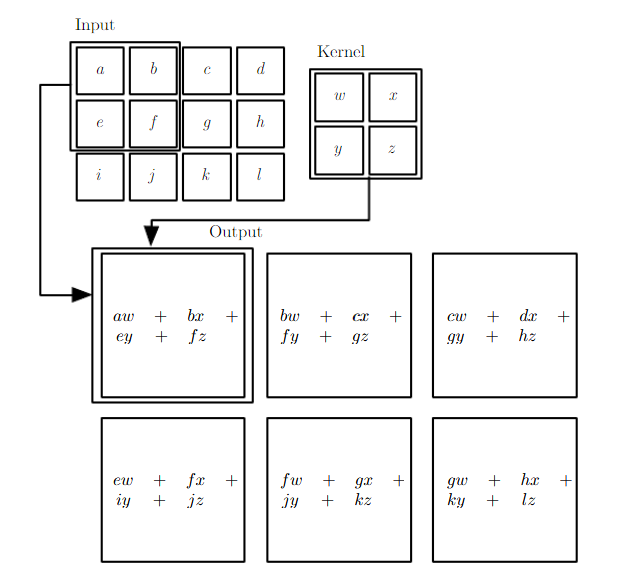
\includegraphics[scale=.35]{../img/cap7_kernel_cnn}}
    \caption{Ejemplo de una convolución 2-D, el valor de \textit{stride} es (1,1) \cite{Goodfellow-et-al-2016}}
\end{figure} \pause 

Una vez extraídas las características mediante la utilización de variados kernel según se requiera, éstas son reubicadas y usadas como entrada para una \textit{feedforward neural network} que se encargará de entregar la salida  correspondiente. 

\end{frame}

\begin{frame}{Redes Neuronales Recurrentes}

Las \textbf{redes neuronales recurrentes} (o \textbf{RNNs}) son una familia de modelos especializados en procesamiento de datos secuenciales, $\bm{x}^{(1)},...,\bm{x}^{(\tau)}$. Las RNNs también comparten parámetros, pero en una forma muy distinta que las CNNs. En una RNN, cada entrada en una etapa es una función de la salida de la etapa anterior. \pause

Se denota por $\bm{h}^{(t)}$ al estado de un sistema din\'amico que involucra una recurrencia conducido por una entrada externa $\bm{x}^{(t)}$:

\begin{equation*}
\bm{h}^{(t)} = f(\bm{h}^{(t-1)}; \bm{x}^{(t)}, \bm{\theta}).
\end{equation*}
\pause

\begin{figure}[H]
\captionsetup{font=small,labelfont=small}
\caption{Ejemplo de una red recurrente sin salida \cite{Goodfellow-et-al-2016}}
\centering
\visible<3->{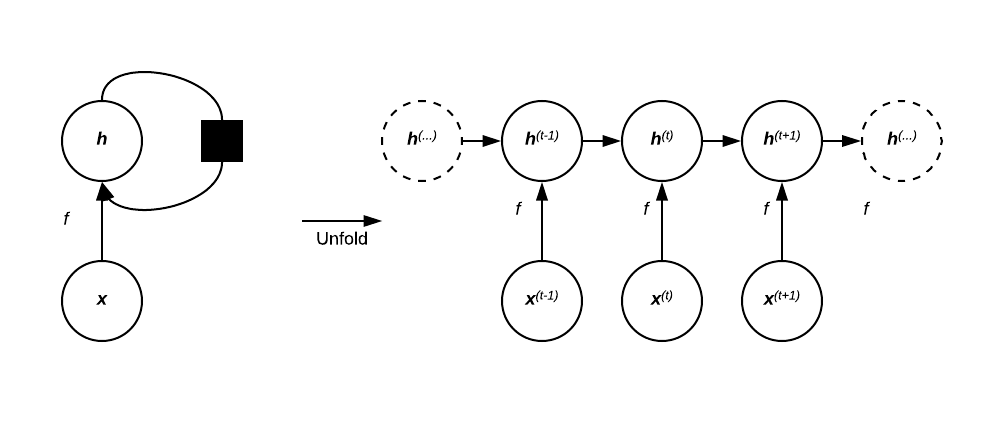
\includegraphics[scale=.3]{../img/cap7_RNN1.png}}
\end{figure}

\end{frame}

\begin{frame}{Redes Neuronales Recurrentes}
Existen varios tipos de RNNs que se han diseñado para distintos fines. \pause

\begin{columns}
  \begin{column}{0.5\textwidth}
    \begin{itemize}
      \item Redes recurrentes que producen una salida en cada instante de tiempo y tienen conexiones entre todas las unidades escondidas \pause
      \item Redes recurrentes que producen una salida en cada instante de tiempo y tienen conexiones entre la salida a la unidad escondida del siguiente instante \pause
      \item Redes recurrentes con conexiones entre las unidad escondidas, que procesan una secuencia entera antes de producir la salida \pause
    \end{itemize}

  \end{column}

  \begin{column}{0.5\textwidth}

    \begin{figure}[H]
    \captionsetup{font=small,labelfont=small}
    \visible<5->{\caption{Red recurrente para el primer ejemplo \cite{Goodfellow-et-al-2016}}}
    \centering
    \visible<5->{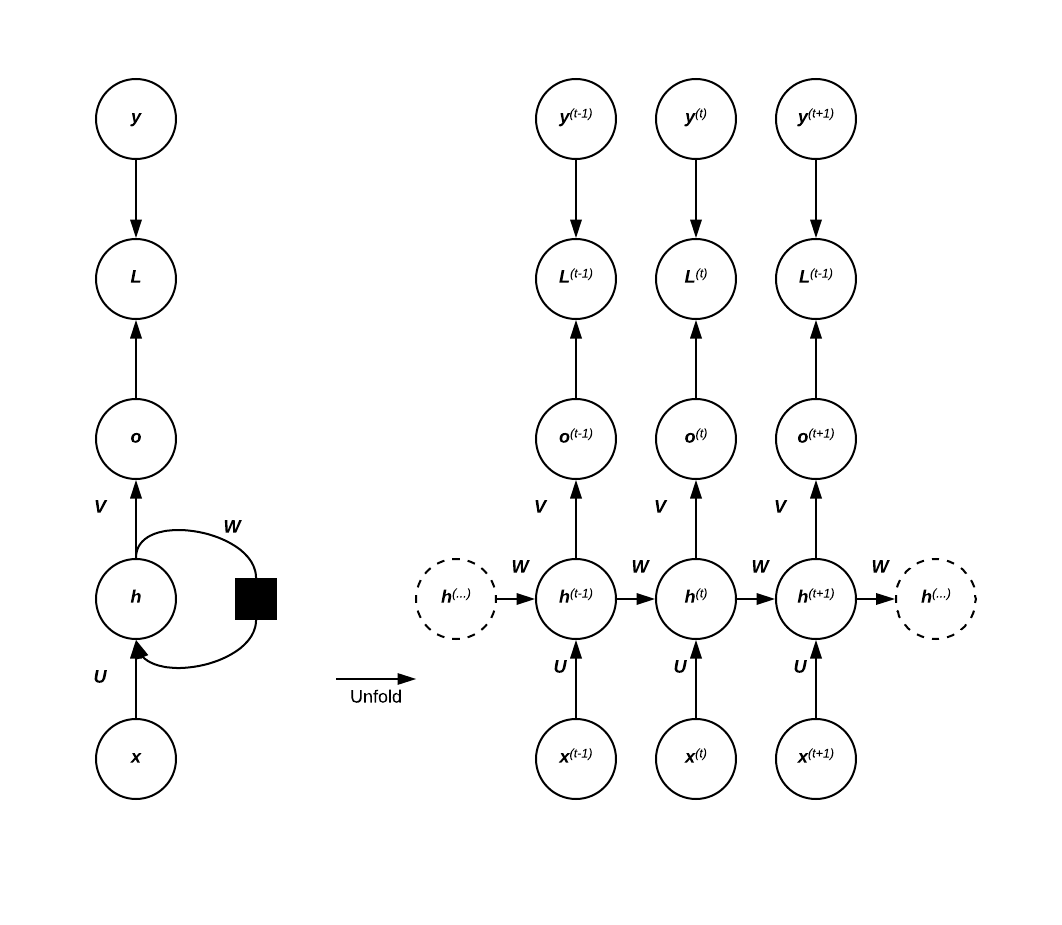
\includegraphics[scale=.2]{../img/cap7_RNN2.png}}
    \end{figure}

  \end{column}

\end{columns}


\end{frame}


\begin{frame}{Autoencoders}
Un \textbf{autoencoder} es una red neuronal que busca replicar la entrada hacia la salida, es decir, busca que la información que entra a la red sea lo más parecida posible a la de salida, para lo cual cuenta con una capa interna $\bm{h} = f(\bm{x})$ (\textbf{encoder}) con menor dimensión que la entrada y que lo codifica (genera una representación de baja dimensión de la entrada) y una función que produce la reconstrucción $\bm{r} = g(\bm{h})$, el \textbf{decoder}. \pause \\

Un autoencoder buscará aprender los \textit{encoder} y \textit{decoder} tales que $g(f(\bm{x})) = \bm{x}$ para todo $\bm{x}$. Como el modelo está forzado a aprender los atributos más importantes para que pueda efectivamente reproducir la entrada en su salida, este aprenderá en general propiedades útiles de los datos de entrenamiento. Los \textit{autoencoders} modernos modelan mappings estocásticos $p_{\textrm{encoder}}(\bm{h}|\bm{x})$ y $p_{\textrm{decoder}}(\bm{x}|\bm{h})$, en vez de funciones determinísticas. \pause

\begin{figure}[H]
\captionsetup{font=small,labelfont=small}
\centering
\visible<3->{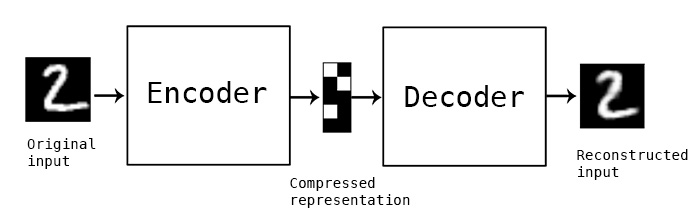
\includegraphics[scale=1.5]{../img/cap7_autoencoder_ejemplo}}
\end{figure}

\end{frame}


\begin{frame}{Redes Generativas Adversariales}

Una \textbf{red generativa adversarial} (o \textbf{GAN}) se basa en un escenario de teoría de juegos, en donde una \textbf{red generadora} debe competir con un adversario. La red generadora produce muestras $\bm{x} = g(\bm{z};\bm{\theta}^{(g)})$, mientras que una \textbf{red discriminadora} trata de distinguir entre muestras obtenidas de los datos de entrenamiento y muestras generadas por la red generadora. El discriminador retorna una probabilidad, $d(\bm{x};\bm{\theta}^{(d)})$, indicando la probabilidad de que $\bm{x}$ sea un dato real y no uno simulado. \pause
 
Para formular el aprendizaje, se describe un juego de suma cero en donde una función $v(\bm{\theta}^{(g)},\bm{\theta}^{(d)})$ determina el pago del discriminador, y el generador recibe $-v(\bm{\theta}^{(g)},\bm{\theta}^{(d)})$ como pago. Así, durante el entrenamiento cada jugador intenta maximizar su propio pago, para que en convergencia se tenga \pause

\begin{equation*}
g^{*} = \textrm{arg} \textrm{min}_{g} \textrm{max}_{d} v(g,d).
\end{equation*} \pause

Esto motiva a que el discriminador aprenda a clasificar correctamente entre muestras reales y falsas y, simulatáneamente, el generador intenta engañar al clasificador para que crea que las muestras generadas son reales. En convergencia, las muestras del generador son indistinguibles de los datos reales. Una motivación del uso de GANs es que cuando $\textrm{max}_{d} v(g,d)$ es convexa en $\bm{\theta}^{(g)}$, el procedimiento asegura la convergencia.


\end{frame}

\begin{frame}{Redes Generativas Adversariales}
\begin{figure}[H]
\captionsetup{font=small,labelfont=small}
\centering
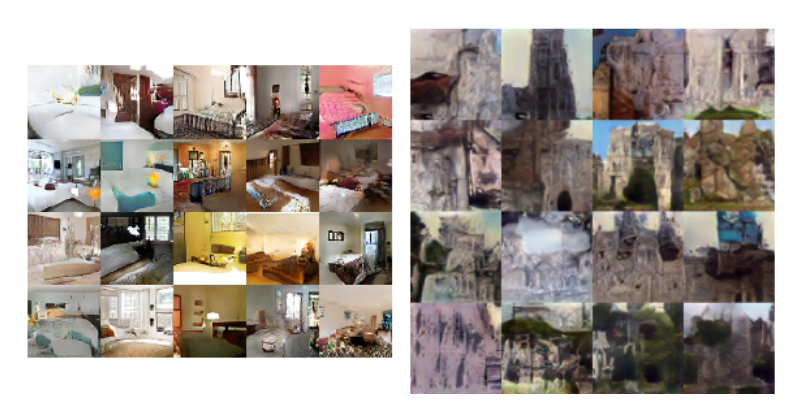
\includegraphics[scale=.7]{../img/cap7_gans.PNG}
\caption{Imágenes generadas por una GAN entrenada con el set de datos LSUN. (Izquierda) Imágenes de dormitorios generadas por el modelo DCGAN (imagen de Radford et al., 2015). (Derecha) Imágenes de iglesias generadas por el modelo LAPGAN (imagen de Denton et al., 2015)}
\end{figure}

\end{frame}

\begin{frame}
  \titlepage
\end{frame}






%Quitar de comentarios apenas se agregue alguna referencia 
\bibliography{../capitulos/referencias} %Bibliografía
\bibliographystyle{apacite}
\end{document} 